%package list
\documentclass{article}
\usepackage[top=3cm, bottom=3cm, outer=3cm, inner=3cm]{geometry}
\usepackage{graphicx}
\usepackage{url}
%\usepackage{cite}
\usepackage{hyperref}
\usepackage{array}
%\usepackage{multicol}
\newcolumntype{x}[1]{>{\centering\arraybackslash\hspace{0pt}}p{#1}}
\usepackage{natbib}
\usepackage{pdfpages}
\usepackage{multirow}
\usepackage{multirow}
\usepackage[T1]{fontenc}
\usepackage{imakeidx}
% Imagenes de costado
\usepackage{wrapfig}
\usepackage{graphicx}

% Modificar URLs
\usepackage{hyperref}
\hypersetup{
    colorlinks=true,
    linkcolor=black,
    filecolor=magenta,      
    urlcolor=blue,
    pdftitle={Overleaf Example},
    pdfpagemode=FullScreen,
    }

\urlstyle{same}

\usepackage[normalem]{ulem}
\useunder{\uline}{\ul}{}

\usepackage[newfloat]{minted}
\usepackage{caption}

\newenvironment{code}{\captionsetup{type=listing}}{}
\SetupFloatingEnvironment{listing}{name=Source Code}

% codigo fuente
\usepackage{listings}
\usepackage{color, colortbl}
\definecolor{dkgreen}{rgb}{0,0.6,0}
\definecolor{gray}{rgb}{0.5,0.5,0.5}
\definecolor{mauve}{rgb}{0.58,0,0.82}
\definecolor{codebackground}{rgb}{0.95, 0.95, 0.92}
\definecolor{tablebackground}{rgb}{0.0, 0.45, 0.63}
\lstset{frame=tb,
	language=bash,
	aboveskip=3mm,
	belowskip=3mm,
	showstringspaces=false,
	columns=flexible,
	basicstyle={\small\ttfamily},
	numbers=none,
	numberstyle=\tiny\color{gray},
	keywordstyle=\color{blue},
	commentstyle=\color{dkgreen},
	stringstyle=\color{mauve},
	breaklines=true,
	breakatwhitespace=true,
	tabsize=3,
	backgroundcolor= \color{codebackground},
}

%%%%%%%%%%%%%%%%%%%%%%%%%%%%%%%%%%%%%%%%%%%%%%%%%%%%%%%%%%%%%%%%%%%%%%%%%%%%
%%%%%%%%%%%%%%%%%%%%%%%%%%%%%%%%%%%%%%%%%%%%%%%%%%%%%%%%%%%%%%%%%%%%%%%%%%%%
\newcommand{\csemail}{vmachacaa@ulasalle.edu.pe}
\newcommand{\csdocente}{MSc. Maribel Molina Barriga}
\newcommand{\cscurso}{Sistemas Operativos}
\newcommand{\csuniversidad}{Universidad La Salle}
\newcommand{\csescuela}{Escuela Profesional de Ingeniería de Software}
\newcommand{\cspracnr}{01}
\newcommand{\cstema}{Planificacion de Procesos}
%%%%%%%%%%%%%%%%%%%%%%%%%%%%%%%%%%%%%%%%%%%%%%%%%%%%%%%%%%%%%%%%%%%%%%%%%%%%
%%%%%%%%%%%%%%%%%%%%%%%%%%%%%%%%%%%%%%%%%%%%%%%%%%%%%%%%%%%%%%%%%%%%%%%%%%%%


\usepackage[english,spanish]{babel}
\usepackage[utf8]{inputenc}
\AtBeginDocument{\selectlanguage{spanish}}
\renewcommand{\figurename}{Figura}
\renewcommand{\refname}{Referencias}
\renewcommand{\tablename}{Tabla} %esto no funciona cuando se usa babel
\AtBeginDocument{%
	\renewcommand\tablename{Tabla}
}

\usepackage{fancyhdr}
\pagestyle{fancy}
\fancyhf{}
\setlength{\headheight}{30pt}
\renewcommand{\headrulewidth}{1pt}
\renewcommand{\footrulewidth}{1pt}
\fancyhead[L]{\raisebox{-0.2\height}{
\includegraphics[width=3cm]{logo_ulasalle (1).png}}}
\fancyhead[C]{}
\fancyhead[R]{\fontsize{7}{7}\selectfont	\csuniversidad \\ \csescuela \\ \textbf{\cscurso} }
\fancyfoot[L]{}
\fancyfoot[C]{Sistemas Operativos}
\fancyfoot[R]{Página \thepage}



\begin{document}

	\vspace*{10px}
	
	\begin{center}	
		\fontsize{17}{17} \textbf{ Trabajo de planificación	}
	\end{center}
	%\centerline{\textbf{\underline{\Large Título: Informe de revisión del estado del arte}}}
	%\vspace*{0.5cm}
	

\renewcommand{\arraystretch}{1.5}
\begin{table}[h]
	\begin{tabular}{|x{4.7cm}|x{4.8cm}|x{4.8cm}|}
		\hline 
		\textbf{DOCENTE} & \textbf{CARRERA}  & \textbf{CURSO}   \\
		\hline 
		\csdocente & \csescuela & \cscurso    \\
		\hline 
	\end{tabular}
\end{table}	

\begin{table}[h]
	\begin{tabular}{|x{4.7cm}|x{4.8cm}|x{4.8cm}|}
		\hline 
		\textbf{GRUPO} & \textbf{TEMA}  & \textbf{DURACIÓN}   \\
		\hline 
		\ 6 & \cstema & 5 horas   \\
		\hline 
	\end{tabular}
\end{table}
\renewcommand{\arraystretch}{1} 
	\section*{Integrantes}
	 	\begin{itemize}
            \item José Carlos Machaca Vera
	 		\item Jhosep Alonso Mollapaza Morocco
	 		\item Patrick Andres Ramirez Santos
	 \end{itemize}
 
	\tableofcontents

\vspace*{\fill}
\section*{Nota}
Para las graficas se considero la notacion xProcesoNumero para
procesos que no se terminan con el quantum disponible y 
-ProcesoNumero para los que si han logrado terminar y no tienen 
que regresar a la cola, ademas estan coloreados de color rojo
y verde respectivamente. Los cambios entre hilos son de color amarillo
para mostrar el tiempo requerido y los espacios de azul son los 
momentos en los que la CPU no esta haciendo ninguna tarea
	

\newpage

\section{SO hilos en espacio de usuario}
En este sistema se dispone de
una biblioteca para la programación con hilos en espacio de usuario. El algoritmo de
planificación de CPU utilizado por el sistema operativo es Round Robin con un quantum de 100
u.t. y un coste por cambio de contexto entre procesos de 20 u.t. El planificador de la biblioteca
de hilos reparte el quantum del proceso entre los hilos utilizando Round Robin con un quantum
para cada hilo de 10 u.t. y sin coste en el cambio de contexto entre sus hilos.

Para ver el archivo completo visitar \href{https://docs.google.com/spreadsheets/d/1Rp1qp1uHB0s8WWKpClNhiJQQU-BFLd2jRRI6iWhH4GQ/edit?usp=sharing}{Esta hoja de calculo} 
en la hoja llamada E1 
\begin{figure}[h]
\caption{Captura parcial de gráfica de planificación 1}
\centering
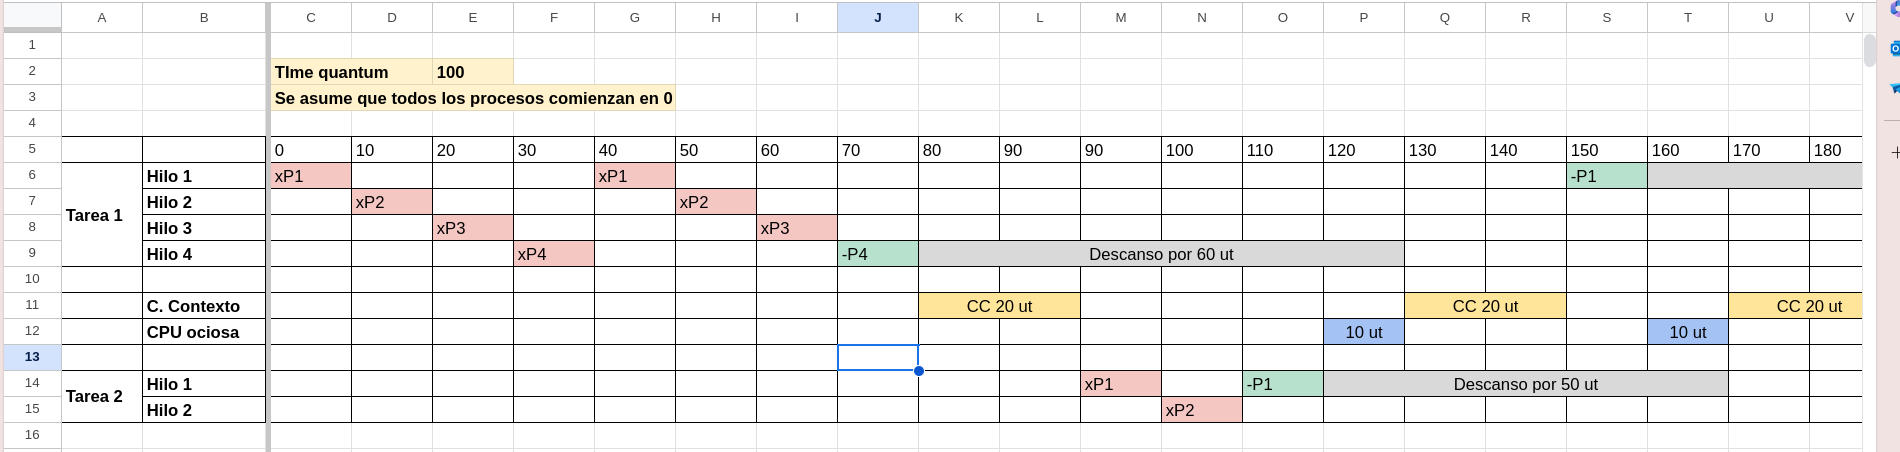
\includegraphics[scale=0.25,clip]{test1.png}
\end{figure}

\begin{center} \textbf{Tabla de tiempos para Tarea 1}
	\newline
	\newline
	\begin{tabular}{||c c c c||} 
	 \hline
	 Hilo & Tiempo Finalizacion & Tiempo Turnaround & Tiempo espera \\ [0.5ex] 
	 \hline\hline
	 1 & 500 & $500 - 0 = 500$ & $500 - (30 + 40) = 430$  \\ 
	 \hline
	 2 & 370 & $370 - 0 = 370$ & $370 - (50) = 320$ \\
	 \hline
	 3 & 310 & $310 - 0 = 370$  & $310 - (30) = 280$ \\
	 \hline
	 4 & 400 & $400 - 0 = 400$ & $400 - (20 + 40) = 360$ \\
	 \hline
	\end{tabular}
\end{center}

\begin{center} \textbf{Tabla de tiempos para Tarea 2}
	\newline
	\newline
	\begin{tabular}{||c c c c||} 
	 \hline
	 Hilo & Tiempo Finalizacion & Tiempo Turnaround & Tiempo espera \\ [0.5ex] 
	 \hline\hline
	 1 & 530 & $530 - 0 = 530$ & $530 - (20 + 60) = 450$  \\ 
	 \hline
	 2 & 470 & $470 - 0 = 470$ & $470 - (40 + 20) = 410$ \\
	\end{tabular}
\end{center}

Entonces los valores a calcular serian los siguientes:
\begin{itemize}
	\item Tiempo medio de espera
	\begin{center}
		$ Promedio\  tiempo\  de\  espera = \frac{430 + 320 + 280 + 360 + 450 + 410}{6} = 375 $
	\end{center}
	\item Tiempo medio de sobrecarga
	\begin{center}
		$ \frac{Cambio\  de\  contexto}{Tiempo\  total} = \frac{140}{530} = 26.42\% $
	\end{center}		
	\item Porcentaje de uso efectivo del CPU
	\begin{center}
		$ \frac{CPU \  ocupada\  con\  hilos}{Tiempo\  total} = \frac{350}{530} = 66.03\% $
	\end{center}
	\item Porcentaje de uso de CPU
	\begin{center}
		$ \frac{CPU \  ocupada}{Tiempo\  total} = \frac{490}{530} = 92.45\% $
	\end{center}
\end{itemize}

\section{SO multitarea con hilos soportados dentro del núcleo}
El sistema operativo
planifica los procesos mediante Round Robin con un quantum de 100 u.t. este tiempo se
distribuye de forma circular entre los hilos de esa tarea en rodajes de 10 u.t. Como el caso
anterior, la única sobrecarga que se considera es el cambio de contexto entre procesos con un
coste de 20 u.t. considere además que las operaciones de E/S de una tarea únicamente bloquean
al hilo que las solicita

Para ver el archivo completo visitar \href{https://docs.google.com/spreadsheets/d/1Rp1qp1uHB0s8WWKpClNhiJQQU-BFLd2jRRI6iWhH4GQ/edit?usp=sharing}{Esta hoja de calculo} 
en la hoja llamada E2 
\begin{figure}[h]
\caption{Captura parcial de grafica de planificación 2}
\centering
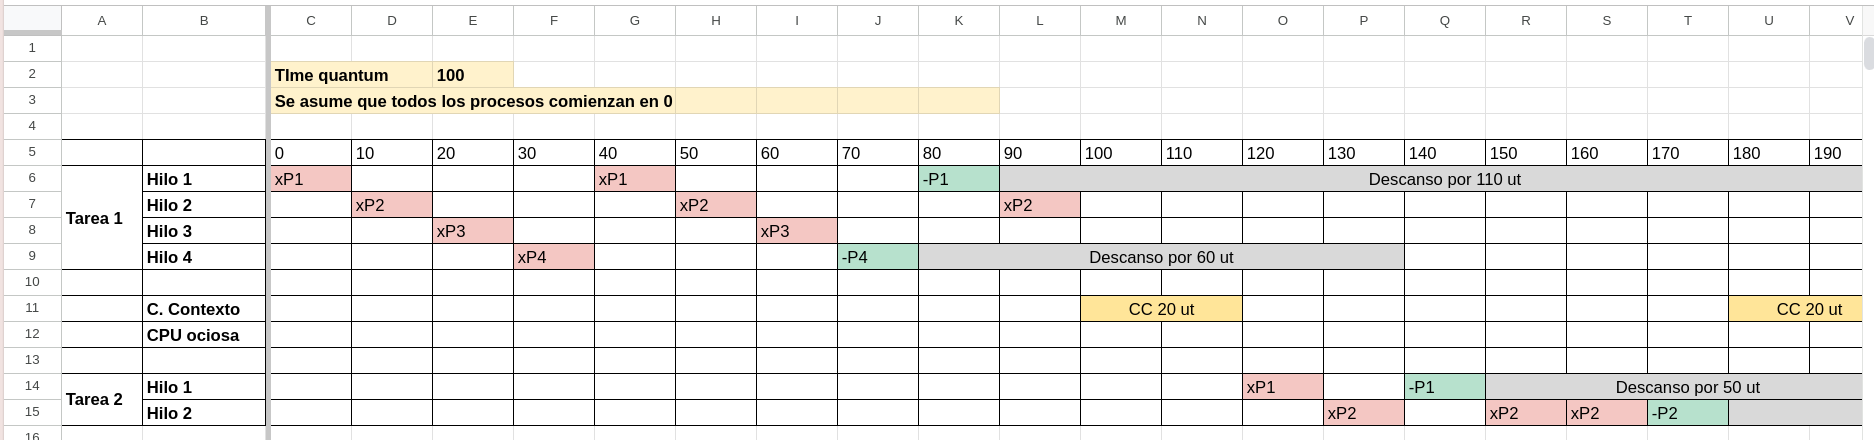
\includegraphics[scale=0.25,clip]{test2.png}
\end{figure}

\begin{center} \textbf{Tabla de tiempos para Tarea 1}
	\newline
	\newline
	\begin{tabular}{||c c c c||} 
	 \hline
	 Hilo & Tiempo Finalizacion & Tiempo Turnaround & Tiempo espera \\ [0.5ex] 
	 \hline\hline
	 1 & 430 & $430 - 0 = 430$ & $430 - (30 + 40) = 360$  \\ 
	 \hline
	 2 & 270 & $270 - 0 = 270$ & $270 - (50) = 220$ \\
	 \hline
	 3 & 210 & $210 - 0 = 210$  & $210 - (30) = 180$ \\
	 \hline
	 4 & 300 & $400 - 0 = 300$ & $300 - (20 + 40) = 240$ \\
	 \hline
	\end{tabular}
\end{center}

\begin{center} \textbf{Tabla de tiempos para Tarea 2}
	\newline
	\newline
	\begin{tabular}{||c c c c||} 
	 \hline
	 Hilo & Tiempo Finalizacion & Tiempo Turnaround & Tiempo espera \\ [0.5ex] 
	 \hline\hline
	 1 & 400 & $400 - 0 = 400$ & $400 - (20 + 60) = 320$  \\ 
	 \hline
	 2 & 360 & $360 - 0 = 360$ & $360 - (40 + 20) = 300$ \\
	\end{tabular}
\end{center}

Entonces los valores a calcular serian los siguientes:
\begin{itemize}
	\item Tiempo medio de espera	
	\begin{center}
		$ Promedio\  tiempo\  de\  espera = \frac{360 + 220 + 180 + 240 + 320 + 300}{6} = 270 $
	\end{center}
	\item Tiempo medio de sobrecarga
	\begin{center}
		$ \frac{Cambio\  de\  contexto}{Tiempo\  total} = \frac{0}{530} = 0\% $
	\end{center}		
	\item Porcentaje de uso efectivo del CPU
	\begin{center}
		$ \frac{CPU \  ocupada\  con\  hilos}{Tiempo\  total} = \frac{350}{430} = 81.40\% $
	\end{center}
	\item Porcentaje de uso de CPU
	\begin{center}
		$ \frac{CPU \  ocupada}{Tiempo\  total} = \frac{430}{430} = 100\% $
	\end{center}
\end{itemize}

\section{Conclusiones}
\begin{enumerate}
	\item  \textbf{Eficiencia en la Gestión de Hilos}: Los sistemas operativos 
	analizados utilizan estrategias de multitarea tanto con hilos en 
	el espacio de usuario como hilos soportados dentro del núcleo, 
	mostrando cómo diferentes enfoques afectan la eficiencia en la 
	gestión de procesos.
	\item  \textbf{Implementación de Round Robin}: Ambos sistemas utilizan el 
	algoritmo de planificación Round Robin, pero difieren en cómo 
	los quanta son asignados y cómo se maneja el cambio de contexto 
	entre hilos y procesos, impactando directamente en la sobrecarga y
	eficiencia del sistema.
	\item  \textbf{Sobrecarga de Cambio de Contexto}: Se observa una diferencia 
	significativa en la sobrecarga debido a los cambios de contexto 
	entre los sistemas, lo que resalta la importancia de una gestión 
	eficiente del cambio de contexto para mejorar el rendimiento 
	general del sistema.
	\item  \textbf{Tiempo de Espera y Turnaround}: Los cálculos de tiempo de 
	espera y tiempo de turnaround proporcionados muestran cómo la 
	distribución del quantum y los costos de cambio de contexto
	afectan el tiempo que un proceso pasa en el sistema, ofreciendo 
	una métrica directa de la experiencia del usuario y eficiencia 
	del sistema.
	\item  \textbf{Uso Efectivo del CPU}: Los porcentajes de uso efectivo del 
	CPU y uso total de CPU indican cuánto del tiempo del procesador 
	se dedica a ejecutar hilos en comparación con estar inactivo o 
	cambiar de contexto, ofreciendo un indicativo de cómo la 
	planificación y la gestión de hilos pueden optimizar el uso 
	del hardware.
	\item  \textbf{Impacto de las Operaciones de E/S}: En el sistema con 
	soporte de hilos dentro del núcleo, las operaciones de E/S 
	bloquean solo al hilo que las solicita, mostrando una ventaja 
	en cuanto a la continuidad de ejecución de los demás hilos, 
	lo que puede resultar en un mejor rendimiento de aplicaciones 
	multitarea.
\end{enumerate}

\section{Anexo 1 - Procedimiento en papel}
\includegraphics*[scale=0.07]{p0.jpg}
\includegraphics*[scale=0.07]{p1.jpg}

\renewcommand{\listfigurename}{Indice de Capturas de Pantalla}
\listoffigures 
\addcontentsline{toc}{section}{\listfigurename} 

\end{document}
